\section{Performance Results with Graphs}

The following sections present performance graphs across the evaluated model presets. We compare PyTorch, serial C++, and our custom parallel CUDA implementation to analyze forward-pass runtime across configurations. For each preset, we include a plot highlighting serial C++ performance as a baseline and the resulting speedup obtained through parallelization.

\begin{table}[H]
\centering
\begin{tabular}{lccccc}
\hline
\textbf{Preset} & \textbf{n\_layer} & \textbf{n\_embd} & \textbf{block\_size} & \textbf{n\_head} & \textbf{steps} \\
\hline
small        & 1 & 64  & 128 & 4  & 200   \\
medium       & 2 & 128 & 128 & 8  & 1000  \\
large        & 4 & 256 & 256 & 8  & 2500  \\
very-large   & 6 & 384 & 512 & 12 & 5000  \\
extra-large  & 8 & 512 & 512 & 16 & 10000 \\
\hline
\end{tabular}
\caption{Model and Name Size Configurations}
\end{table}

\begin{figure}[H]
\centering

\begin{subfigure}{0.48\textwidth}
\centering
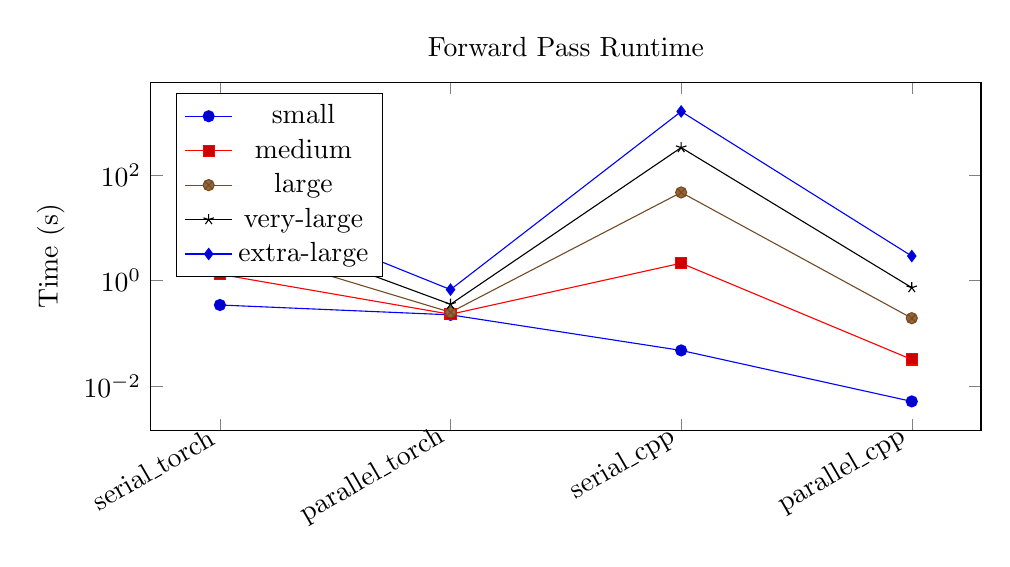
\begin{tikzpicture}
\begin{axis}[
title={Forward Pass Runtime},
ylabel={Time (s)},
ymode=log,
symbolic x coords={serial\_torch,parallel\_torch,serial\_cpp,parallel\_cpp},
xtick=data,
x tick label style={rotate=30,anchor=east},
legend pos=north west,
width=\textwidth,
height=6cm
]

\addplot coordinates {(serial\_torch,0.3464)(parallel\_torch,0.2256)(serial\_cpp,0.0479)(parallel\_cpp,0.0052)};
\addlegendentry{small}

\addplot coordinates {(serial\_torch,1.3181)(parallel\_torch,0.2311)(serial\_cpp,2.1390)(parallel\_cpp,0.0323)};
\addlegendentry{medium}

\addplot coordinates {(serial\_torch,5.2244)(parallel\_torch,0.2523)(serial\_cpp,46.5978)(parallel\_cpp,0.1949)};
\addlegendentry{large}

\addplot coordinates {(serial\_torch,14.5409)(parallel\_torch,0.3575)(serial\_cpp,328.4692)(parallel\_cpp,0.7374)};
\addlegendentry{very-large}

\addplot coordinates {(serial\_torch,38.6489)(parallel\_torch,0.6767)(serial\_cpp,1582.5279)(parallel\_cpp,2.9164)};
\addlegendentry{extra-large}

\end{axis}
\end{tikzpicture}
\caption{Forward pass runtime across presets}
\end{subfigure}
\hfill
\begin{subfigure}{0.48\textwidth}
\centering
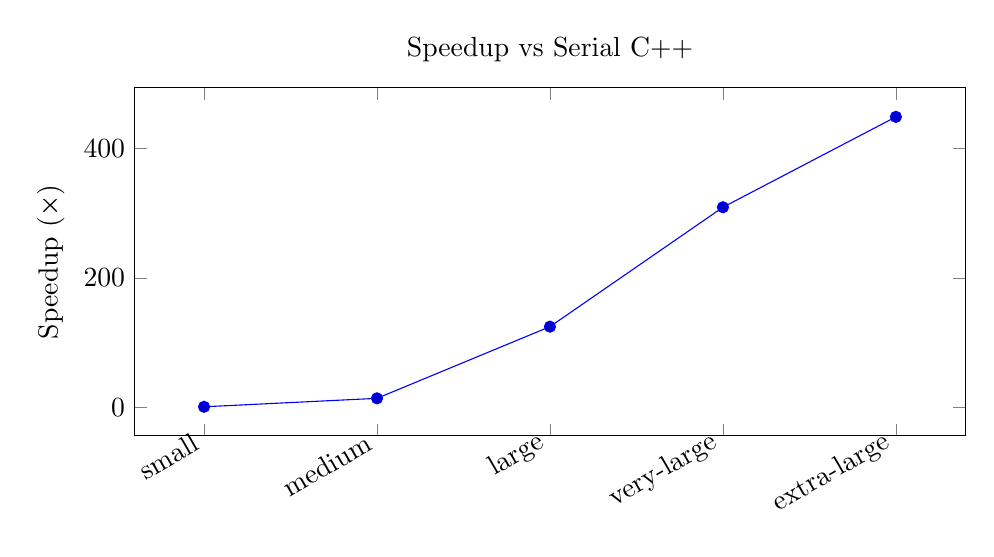
\begin{tikzpicture}
\begin{axis}[
title={Speedup vs Serial C++},
ylabel={Speedup (×)},
symbolic x coords={small,medium,large,very-large,extra-large},
xtick=data,
x tick label style={rotate=30,anchor=east},
width=\textwidth,
height=6cm
]

\addplot coordinates {(small,0.57)(medium,13.65)(large,124.55)(very-large,309.30)(extra-large,449.13)};

\end{axis}
\end{tikzpicture}
\caption{Parallel speedup over serial C++}
\end{subfigure}

\caption{Performance comparison across model size presets}
\label{fig:presets_combined}

\end{figure}

% ================= NAMES =================

\begin{table}[H]
\centering
\begin{tabular}{lccccc}
\hline
\textbf{Preset} & \textbf{n\_layer} & \textbf{n\_embd} & \textbf{block\_size} & \textbf{n\_head} & \textbf{steps} \\
\hline
names-1k   & 1 & 64  & 512 & 4 & 1000  \\
names-5k   & 1 & 64  & 512 & 4 & 5000  \\
names-10k  & 1 & 64  & 512 & 4 & 10000 \\
names-20k  & 2 & 128 & 512 & 8 & 20000 \\
names-30k  & 2 & 128 & 512 & 8 & 30000 \\
\hline
\end{tabular}
\caption{Name Size Configurations}
\end{table}

\begin{figure}[H]
\centering

\begin{subfigure}{0.48\textwidth}
\centering
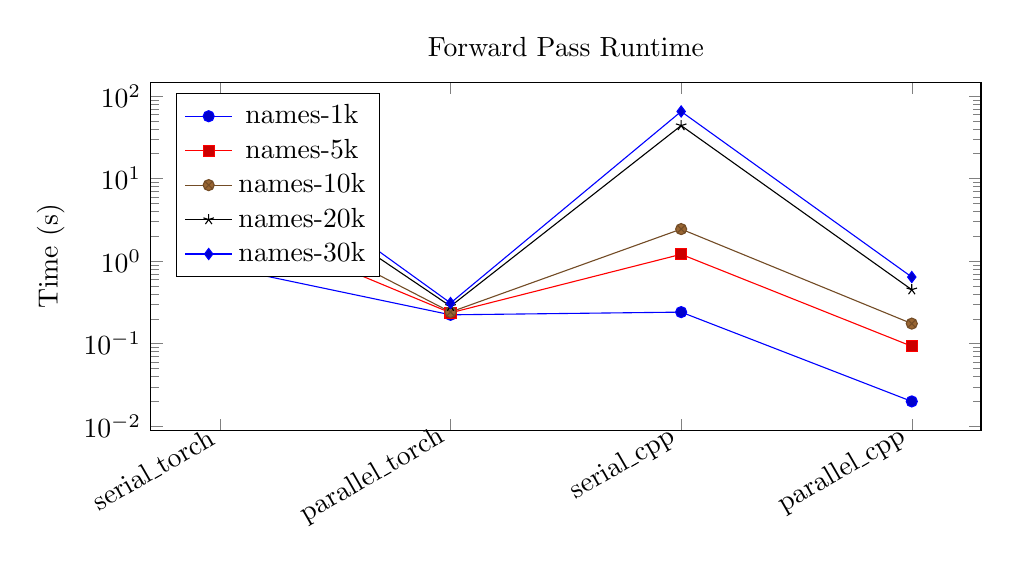
\begin{tikzpicture}
\begin{axis}[
title={Forward Pass Runtime},
ylabel={Time (s)},
ymode=log,
symbolic x coords={serial\_torch,parallel\_torch,serial\_cpp,parallel\_cpp},
xtick=data,
x tick label style={rotate=30,anchor=east},
legend pos=north west,
width=\textwidth,
height=6cm
]

\addplot coordinates {(serial\_torch,0.8637)(parallel\_torch,0.2239)(serial\_cpp,0.2414)(parallel\_cpp,0.0200)};
\addlegendentry{names-1k}

\addplot coordinates {(serial\_torch,3.4358)(parallel\_torch,0.2367)(serial\_cpp,1.2110)(parallel\_cpp,0.0931)};
\addlegendentry{names-5k}

\addplot coordinates {(serial\_torch,6.6577)(parallel\_torch,0.2420)(serial\_cpp,2.4464)(parallel\_cpp,0.1752)};
\addlegendentry{names-10k}

\addplot coordinates {(serial\_torch,21.7865)(parallel\_torch,0.2841)(serial\_cpp,43.8700)(parallel\_cpp,0.4510)};
\addlegendentry{names-20k}

\addplot coordinates {(serial\_torch,32.2511)(parallel\_torch,0.3111)(serial\_cpp,65.0316)(parallel\_cpp,0.6425)};
\addlegendentry{names-30k}

\end{axis}
\end{tikzpicture}
\caption{Forward pass runtime across name sizes}
\end{subfigure}
\hfill
\begin{subfigure}{0.48\textwidth}
\centering
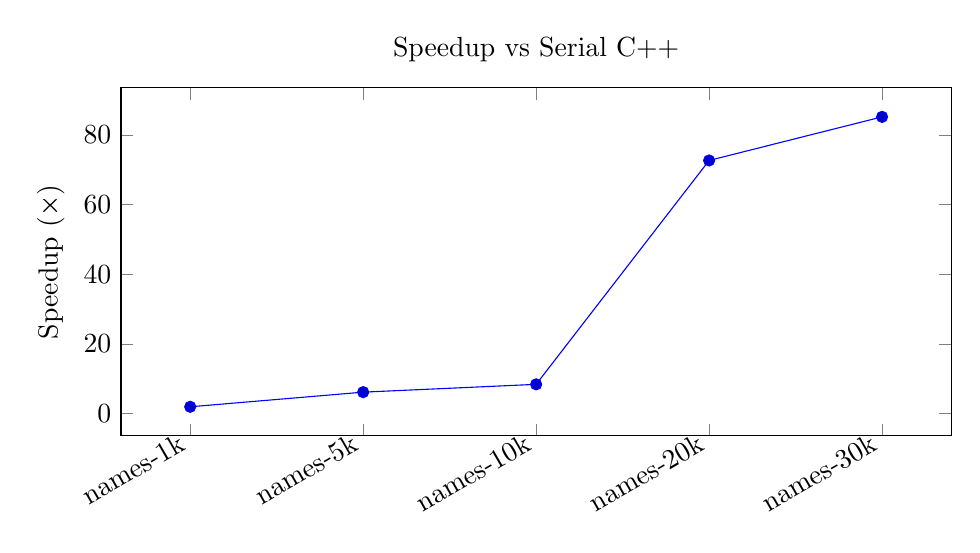
\begin{tikzpicture}
\begin{axis}[
title={Speedup vs Serial C++},
ylabel={Speedup (×)},
symbolic x coords={names-1k,names-5k,names-10k,names-20k,names-30k},
xtick=data,
x tick label style={rotate=30,anchor=east},
width=\textwidth,
height=6cm
]

\addplot coordinates {(names-1k,1.96)(names-5k,6.16)(names-10k,8.40)(names-20k,72.63)(names-30k,85.14)};

\end{axis}
\end{tikzpicture}
\caption{Parallel speedup over serial C++}
\end{subfigure}

\caption{Performance comparison across dataset (name) sizes}
\label{fig:names_combined}

\end{figure}

% ================= MODEL =================

\begin{table}[H]
\centering
\begin{tabular}{lccccc}
\hline
\textbf{Preset} & \textbf{n\_layer} & \textbf{n\_embd} & \textbf{block\_size} & \textbf{n\_head} & \textbf{steps} \\
\hline
model-small-5k        & 1 & 64  & 512 & 4  & 5000 \\
model-medium-5k       & 2 & 128 & 512 & 8  & 5000 \\
model-large-5k        & 4 & 256 & 512 & 8  & 5000 \\
model-very-large-5k   & 6 & 384 & 512 & 12 & 5000 \\
model-extra-large-5k  & 8 & 512 & 512 & 16 & 5000 \\
\hline
\end{tabular}
\caption{Model Size Configurations}
\end{table}

\begin{figure}[H]
\centering

\begin{subfigure}{0.48\textwidth}
\centering
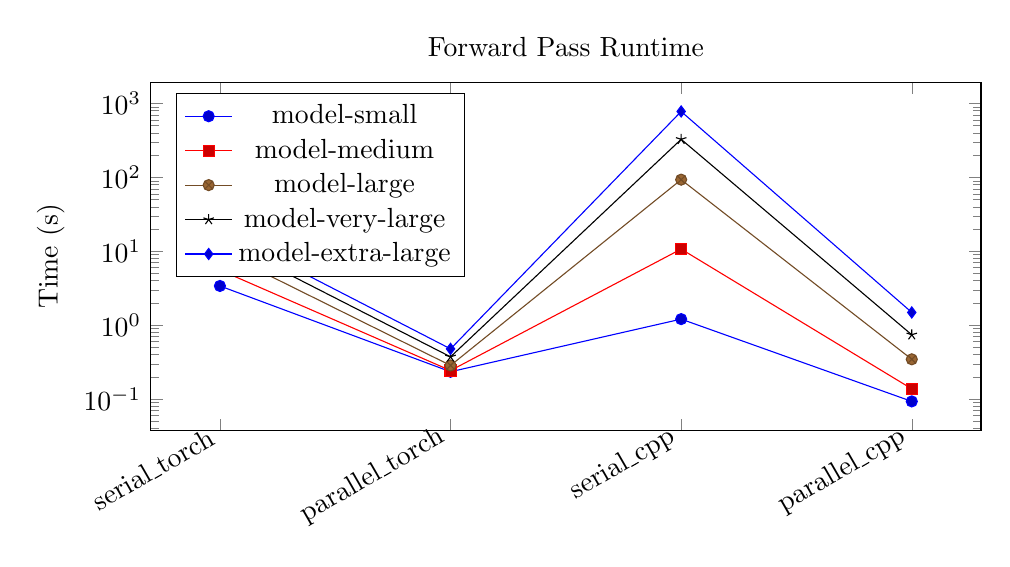
\begin{tikzpicture}
\begin{axis}[
title={Forward Pass Runtime},
ylabel={Time (s)},
ymode=log,
symbolic x coords={serial\_torch,parallel\_torch,serial\_cpp,parallel\_cpp},
xtick=data,
x tick label style={rotate=30,anchor=east},
legend pos=north west,
width=\textwidth,
height=6cm
]

\addplot coordinates {(serial\_torch,3.3999)(parallel\_torch,0.2348)(serial\_cpp,1.2103)(parallel\_cpp,0.0932)};
\addlegendentry{model-small}

\addplot coordinates {(serial\_torch,5.5876)(parallel\_torch,0.2438)(serial\_cpp,10.7280)(parallel\_cpp,0.1379)};
\addlegendentry{model-medium}

\addplot coordinates {(serial\_torch,10.0759)(parallel\_torch,0.2857)(serial\_cpp,93.2595)(parallel\_cpp,0.3460)};
\addlegendentry{model-large}

\addplot coordinates {(serial\_torch,14.6363)(parallel\_torch,0.3737)(serial\_cpp,327.6338)(parallel\_cpp,0.7426)};
\addlegendentry{model-very-large}

\addplot coordinates {(serial\_torch,19.3169)(parallel\_torch,0.4789)(serial\_cpp,779.8755)(parallel\_cpp,1.4909)};
\addlegendentry{model-extra-large}

\end{axis}
\end{tikzpicture}
\caption{Forward pass runtime across model sizes}
\end{subfigure}
\hfill
\begin{subfigure}{0.48\textwidth}
\centering
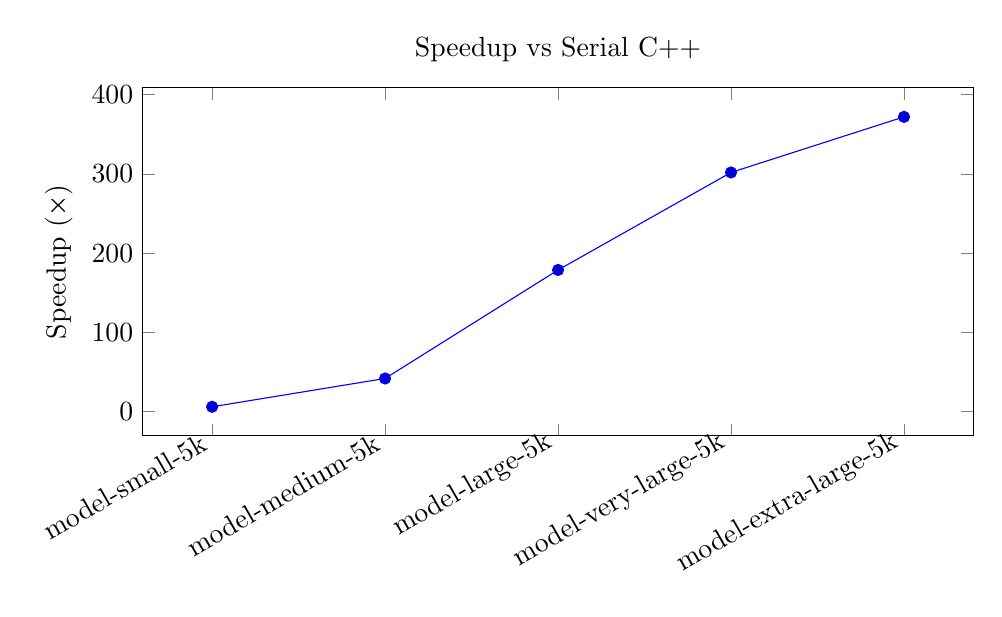
\begin{tikzpicture}
\begin{axis}[
title={Speedup vs Serial C++},
ylabel={Speedup (×)},
symbolic x coords={
model-small-5k,model-medium-5k,model-large-5k,model-very-large-5k,model-extra-large-5k},
xtick=data,
x tick label style={rotate=30,anchor=east},
width=\textwidth,
height=6cm
]

\addplot coordinates {
(model-small-5k,6.22)
(model-medium-5k,41.94)
(model-large-5k,178.73)
(model-very-large-5k,301.69)
(model-extra-large-5k,371.79)
};

\end{axis}
\end{tikzpicture}
\caption{Parallel speedup over serial C++}
\end{subfigure}

\caption{Performance comparison across model scaling (fixed dataset size)}
\label{fig:model_combined}

\end{figure}